\documentclass{article}
\usepackage[english]{babel}
\usepackage{setspace}
\usepackage[letterpaper,top=2cm,bottom=2cm,left=3cm,right=3cm,marginparwidth=1.75cm]{geometry}
\usepackage{amsmath}
\usepackage{graphicx}
\usepackage[colorlinks=true, allcolors=blue]{hyperref}
\usepackage{amsmath}
\usepackage{siunitx}

\title{Investigation into the electrical resistance resulting from different lengths of constantan wire.}
\author{Eric D’Urso}
\begin{document}
\maketitle

\doublespacing
\begin{abstract}
The target of this study is to explore the relationship between the length of a wire and its resistance. Constantan wire was used in the experiment as it provides more uniform resistance than standard wire. The experiment involved a simple circuit with a variable length of constantan wire. Current and electrical potential were measured at various points to determine resistance. Ultimately, the experiment yielded a constant value of resistivity (in ohms per meter, $\frac{\Omega}{m}$) that showed a directly proportional relationship between the length of the wire and its resistance.
\end{abstract}

\section{Introduction}
\label{sec:intro}

I have a tendency trip circuit breakers. Recently, while using a new electric snowblower to clear my driveway, I tripped another breaker. Ultimately, the reason for this turned out to be that the extension cable I was using (16 gauge) was too small (had too much resistance) for the current required by the snowblower. It seems the resistivity of a wire is dependent on its thickness (or gauge) since a different, 12 gauge extension cable did not result in the same outcome. This incident held an important lesson: not all wires are able to conduct charge in the same way. This fact yields an important question: what other factors affect the resistivity of a wire?

In addition to the thickness of a wire, the length of a wire is likely to affect its resistance. In a similar manner to how the volume of a container affects the pressure, I would hypothesize that the length of wire is directly proportional to its resistance since the further the electrical current must travel, the more the electrons would have to collide with one another, causing some back-drive, or resistance, in the circuit.

The length of electrical wire is the subject of this paper. The aim of the experiment is to investigate the relationship between the length of an electrical wire and its ability to function. More specifically, this paper will focus on how the length of a wire can affect the resistance it produces on electrical current. A simple DC circuit will be constructed to test this by measuring the electrical current and potential through a known length of wire. Resistance will then be calculated via \hyperref[sec:ohm]{Ohm's Law} (which defines a relationship between potential, current, and resistance), and a determination will be made as to the relationship between length of wire and its resistance.

Since standard, copper wire conducts very well and contains a negligible amount of resistance in smaller circuits (as discussed in \hyperref[sec:wires]{this section}), very long lengths of wire would be required for the experiment to yield realistic and easily-measurable results. Instead of standard wire, constantan wire will be used. Constantan wire is composed of roughly $55\%$ copper and $45\%$ nickel, and is commonly used in heating elements due to its resistive properties \cite{sis}.

\subsection{Research Question}

How does the length of constantan wire affect its resistance?

\subsection{Hypothesis}
\label{sec:hypot}

There will be a directly proportional relationship between the length of the constantan wire and its resistance.

\section{Methods}

\subsection{Materials}
This experiment utilizes the materials described in the list below. All materials specified were tested before use.

\begin{enumerate}
    \item Voltmeter (INNOVA 3320 Auto-Ranging Digital Multimeter)
    \item Ammeter (INNOVA 3320 Auto-Ranging Digital Multimeter)
    \item Variable Resistor - Intention of this component is to limit the current flowing through the wire slightly so it does not over heat.
    \item Wire - Wires tested for continuity with a multi-meter before usage.
    \item Constantan Wire - 32 gauge wire (ø0.2mm)
    \item Batteries - Circuit will contain 2 1.5V D batteries. Voltage of batteries was measured before and throughout the experiment to ensure there was negligible variability in the batteries.
    \item Battery Holders - Tested for continuity before use to ensure proper connections to batteries.
    \item Meter stick
\end{enumerate}

\subsection{Circuit Layout}
A circuit diagram used in the experiment is shown in Figure 1. The length of the constantan wire is changed throughout the experiment.

\begin{figure}
\centering
\includegraphics[width=0.9\textwidth]{circuit.png}
\caption{\label{fig:circuit}Complete circuit diagram.}
\end{figure}

The circuit was tested at several points for continuity, potential, and current before the experiment was started to ensure it was functioning correctly. The constantan wire was connected to the voltmeter and wires by wrapping the constantan wire once around the probes of the voltmeter, and clamping it down with the clip on the wire. Figure 2 shows this in more detail.

\begin{figure}
\centering
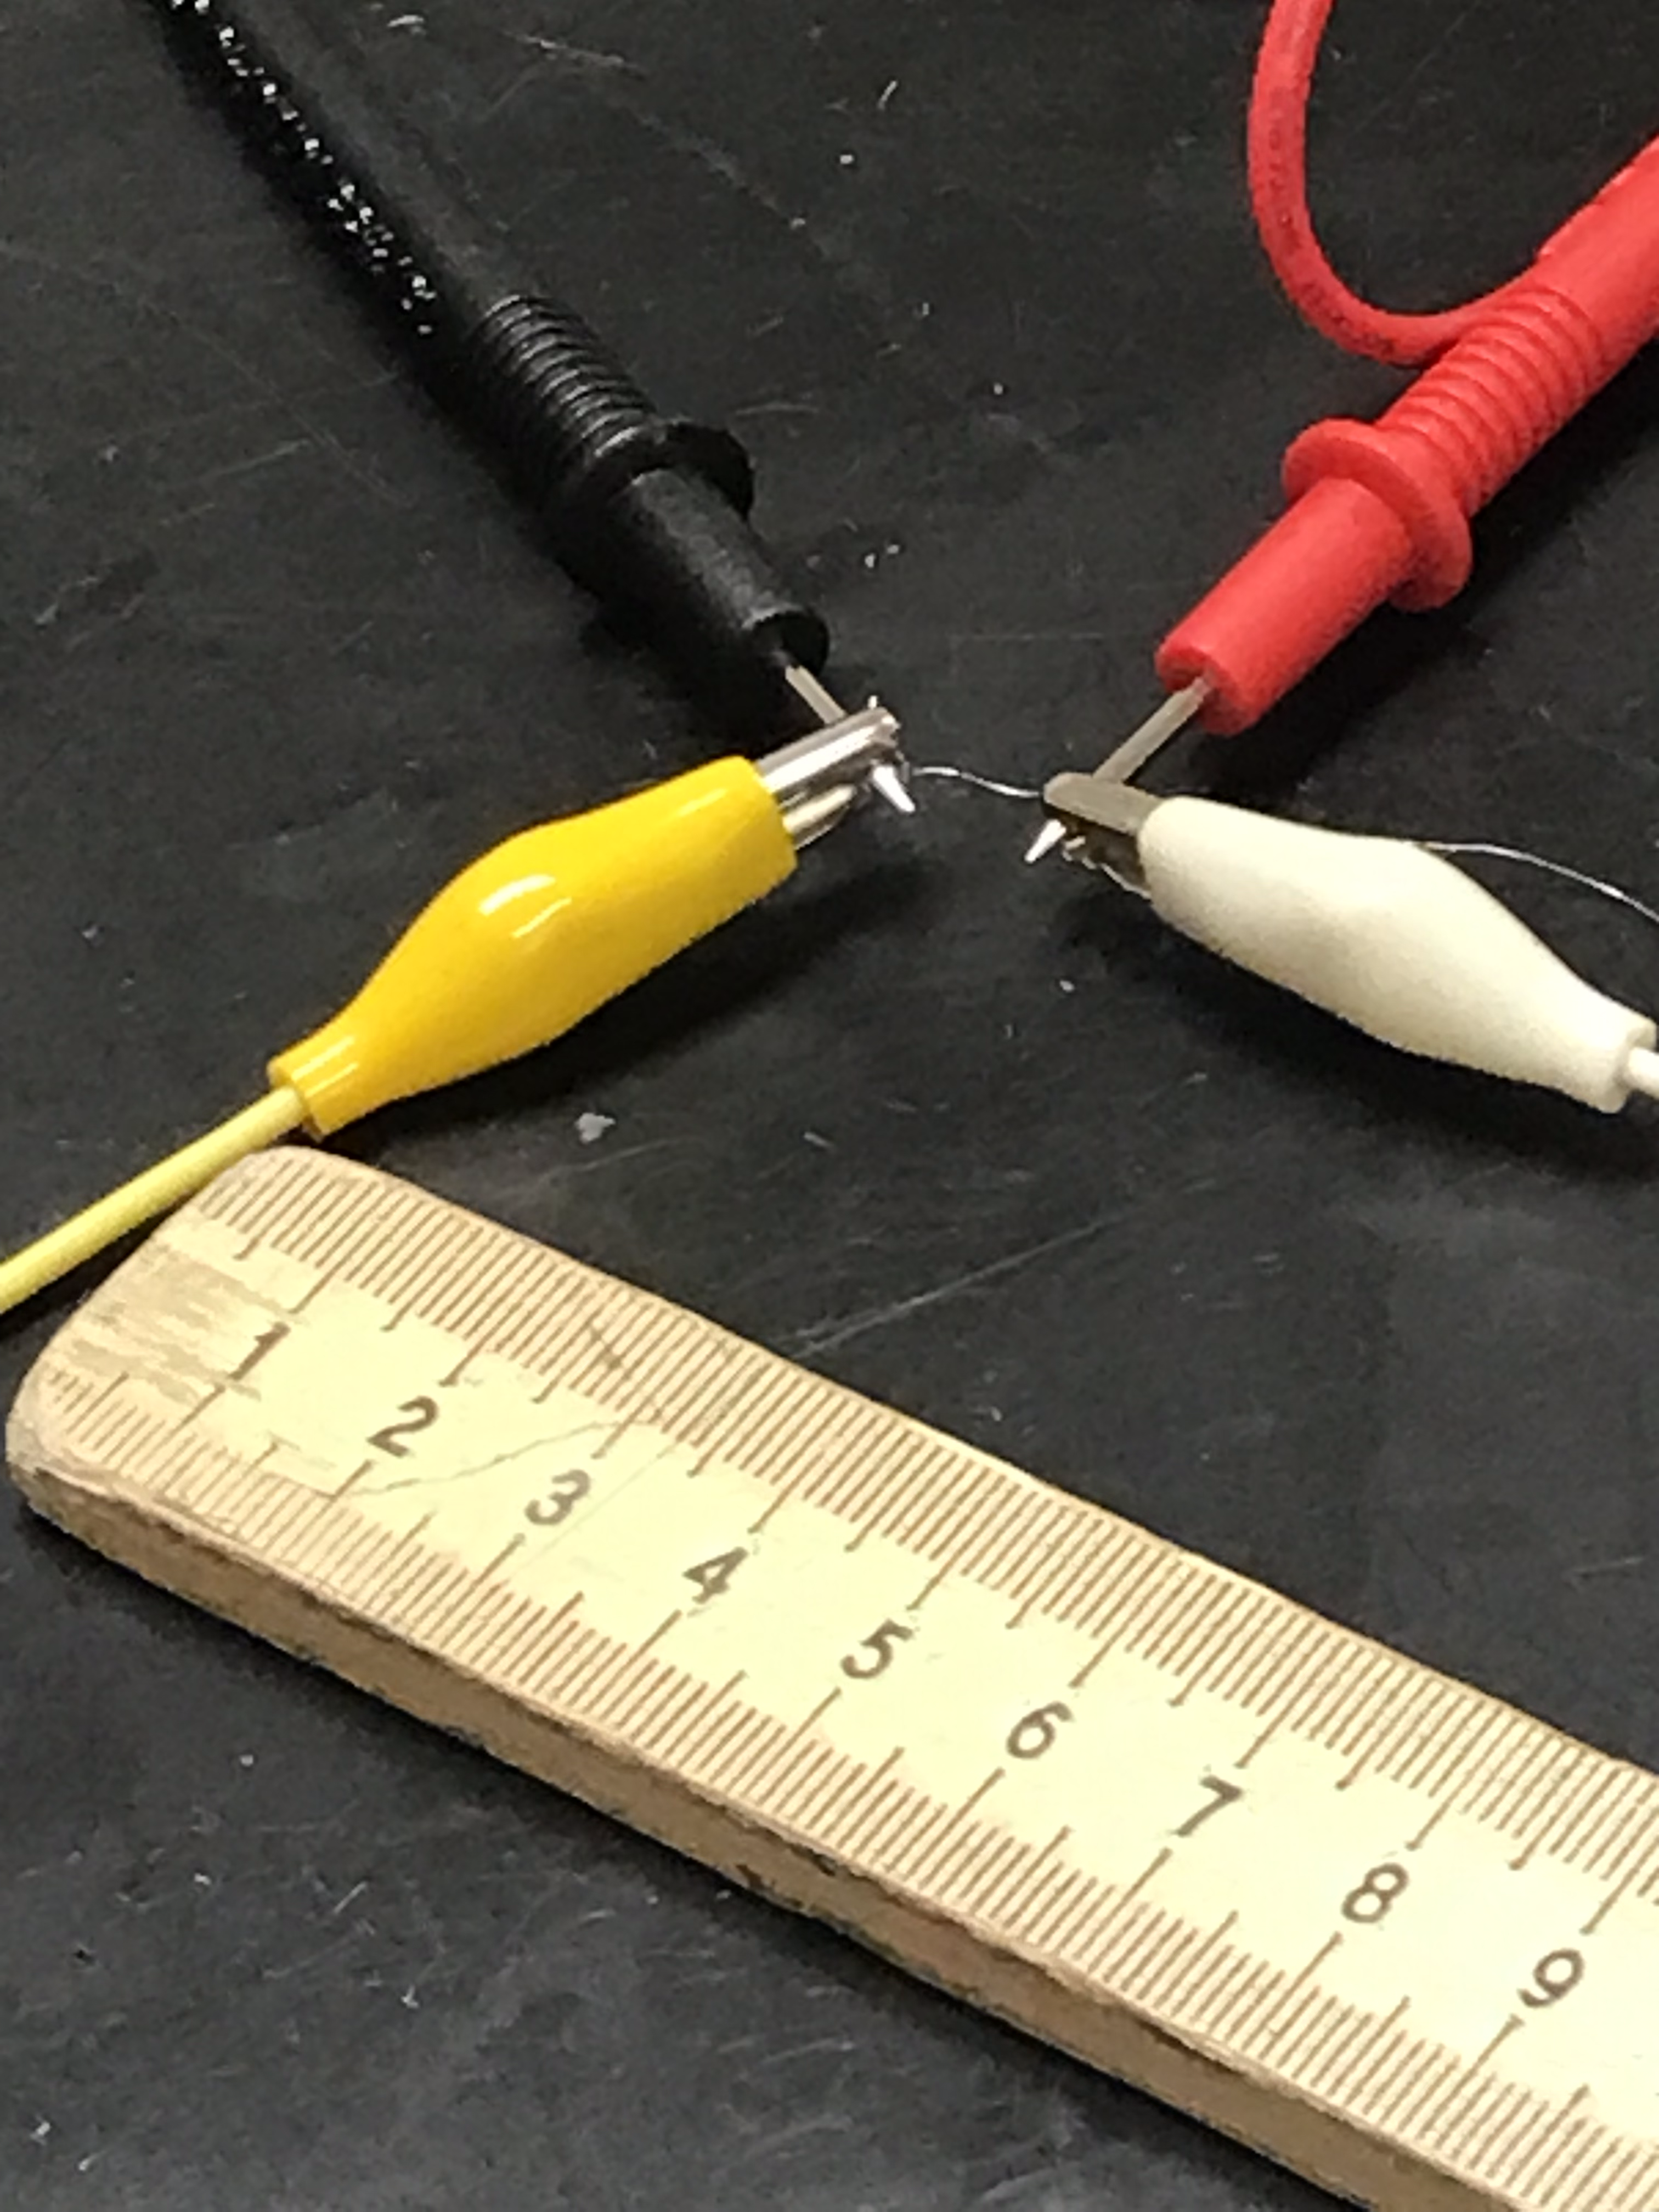
\includegraphics[width=0.5\textwidth]{wire.png}
\caption{\label{fig:wire}Connection of 0.01 m constantan wire to probes and wires.}
\end{figure}

\subsubsection{Safety concerns in experimental procedures}
\label{sec:safe}

Constantan wire is used in heating elements because it heats up when in a circuit with a large amount current \cite{sis}. Due to this, a variable resistor was added to the circuit. Before the experiment was conducted, the variable resistor was tuned so the constantan wire did not heat up to the touch. The resistance induced on the circuit by the variable resistor was not changed between trials. When the trials were being conducted, the circuit was only closed for a short period of time long enough to gather measurements.

\subsection{Procedure}

After the circuit is checked to ensure its proper function, the constantan wire was connected at a pre-determined length. The switch was then switched on to complete the circuit, and the potential across the wire and the current was measured. The switch was then turned off to prevent the constantan wire from overheating. The measurements for potential (measured in volts) and current (measured in amperes) was then entered into a spreadsheet, and resistance (measured in ohms) was calculated via \hyperref[sec:ohm]{Ohm’s Law}.

\subsection{Ohm's Law}
\label{sec:ohm}

Ohm’s Law describes a relationship between electrical potential, current, and resistance. The equation is as follows:

\begin{equation}
    E=IR
\end{equation}

Where \begin{math}E\end{math} denotes potential (volts), \begin{math}I\end{math} denotes current (amperes), and \begin{math}R\end{math} denotes resistance (ohms). To calculate resistance, the equation can be arranged as follows:

\begin{equation}
    R=\frac{E}{I}
\end{equation}

Since potential and current are the measured variables, resistance will be calculated with this formula in an Excel spreadsheet.

\subsection{Variables and constants}

In this experiment, the length of the wire served as the independent variable, with resistance (via voltage and current) as the dependent variable. Other constants throughout the experiment include the lengths and types of wire used to connect the rest of the circuit, the components of the circuit themselves (battery, battery holders, variable resistor, voltmeter, and ammeter) as well as the surface on which the experiment was conducted (a non-conductive tabletop).

Additionally, the voltage of the batteries was held constant with negligible variability throughout the experiment. Resistance induced on the circuit by the variable resistor was not changed after the variable resistor was set for \hyperref[sec:safe]{safety concerns}.

\section{Results}

The results of the experiment are detailed in Table 1. Resistance was calculated from potential and current with Ohm's Law. Figure 3 shows a graphical representation on a scatter plot with a trendline.

\begin{table}[]
\centering
\begin{tabular}{|l|l|l|l|}
\hline
Wire Length (m) & Potential (V) & Current (A) & Resistance ($\Omega$)  \\
$\pm0.005m$    & $\pm0.8\%$    & $\pm1.0\%$ & $\pm1.8\%$ \\
\hline
0.01           & 0.047         & 0.13        & 0.36      \\
0.05           & 0.099         & 0.11        & 0.90      \\
0.10           & 0.206         & 0.09        & 2.29      \\
0.15           & 0.244         & 0.09        & 2.71      \\
0.20           & 0.317         & 0.09        & 3.52      \\
0.25           & 0.371         & 0.09        & 4.12      \\
0.30           & 0.452         & 0.09        & 5.02      \\
0.40           & 0.596         & 0.09        & 6.62      \\
0.50           & 0.750         & 0.09        & 8.33      \\
0.75           & 0.950         & 0.08        & 11.88     \\
1.00           & 1.020         & 0.06        & 17.00     \\
\hline
\end{tabular}
\caption{\label{tab:results}Experiment data.}
\end{table}

\begin{figure}
\centering
\includegraphics[width=1.0\textwidth]{graph.png}
\caption{\label{fig:graph}Visual graph of data with trendline (resistivity), error bars, and maximum/minimum resistivity lines.}
\end{figure}

There is a linear relationship between the length of the constantan wire and its resistance. The raw trendline for this data is:

\begin{equation}
    R = 16.67\frac{\Omega}{m} l + 0.182\Omega
\end{equation}

Where $R$ represents resistance ($\Omega$) and $l$ represents the length of the constantan wire ($m$). Since the \begin{math}0.1818\Omega\end{math} is less than \begin{math}5\%\end{math} of the highest amount of resistance, this value can be considered negligible. See \hyperref[sec:error]{causes of experimental variability} for a discussion of possible causes of this inconsistency. This brings the overall relationship between the constantan wire's length and resistance to 

\begin{equation}
    R = 16.67\frac{\Omega}{m} l
\end{equation}

The key number in this relationship is $16.67\frac{\Omega}{m}$, which is the resistivity of the constantan wire. Resistivity of a wire will be denoted with $\rho$, making the following equation true (see \hyperref[sec:res]{Uncertainty in Resistivity} for a detailed calculation of the uncertainty of this value): 

\begin{equation}
    \rho = 16.67\frac{\Omega}{m} \pm 0.32\frac{\Omega}{m}
\end{equation}

\subsection{Analysis of uncertainties}

\subsubsection{Uncertainty in data collection}

Based on the measuring instrument used and the manner in which it was used, length measurements of the constantan wire were taken to roughly $\pm0.005m$. 

Per the user's manual \cite{man} of the INNOVA 3320 Auto-Ranging Digital Multimeter used in the experiment, the precision of the measurements of direct current potential is listed at $\pm0.8\%$ of the measured value. Using a data point from Table 1, the uncertainty of the potential measurement can be found as follows (note that in all equations below, uncertainty is denoted with the letter $U$):

\begin{equation}
    U_E = 0.047V \times \pm0.8\% = \pm\num{3.8e-4}V
\end{equation}

Since the precision of the current readings is listed at $\pm1.0\%$ of the measured value, a similar calculation can be made with the same data point to determine the uncertainty of the current measurement.

\begin{equation}
    U_I = 0.13A \times \pm1.0\% = \pm\num{1.3e-3}A
\end{equation}

The uncertainty in the resistance calculation can be found by multiplying the calculated resistance value by the sum of both the potential and current uncertainties. For the data point used above, this would look like:

\begin{equation}
    U_R = 0.36\Omega \times (\pm0.8\% + \pm1.0\%) = \pm\num{6.5e-3}\Omega
\end{equation}

\subsubsection{Uncertainty in resistivity}
\label{sec:res}

The final uncertainty value relevant to this experiment is the resistivity value. The minimum and maximum resistivity values can the be calculated with the error bars for resistance from the first and last data points. These values are also reflected on the graph in \hyperref[fig:graph]{Figure 3}.

\begin{equation}
    \rho_{max} = 17.12\frac{\Omega}{m}    
\end{equation}

\begin{equation}
    \rho_{min} = 16.49\frac{\Omega}{m}    s
\end{equation}

The resistivity uncertainty then becomes half of the difference of these values:

\begin{equation}
    U_{\rho} = \pm\frac{\rho_{max} - \rho_{min}}{2} = \pm\frac{17.12\frac{\Omega}{m} - 16.49\frac{\Omega}{m}}{2} = \pm 0.32\frac{\Omega}{m}
\end{equation}


\section{Discussion}

\subsection{Conclusion}

The experiment proved the \hyperref[sec:hypot]{hypothesis} correct by showing a clear proportional relationship between the length of the constantan wire and its resistance and determining a constant value of resistivity. 

\subsection{Is constantan wire representative of standard wire?}
\label{sec:wires}

One question that arises from this experiment is the potential for differences in the results had standard wires been used throughout the circuit as opposed to the variable-length constantan wire.

Constantan wire and standard wire are very similar in the regard that they are both intended to conduct electricity, but constantan wire is uniformly less conductive than standard wire, which is why constantan wire has more resistance than standard wire \cite{sis}. Since all conductive materials still have some degree of measurable resistance, the constantan wire is representative of standard wire in terms of demonstrating resistance, however standard wire will show significantly less, if not negligible, deviation at the distances measured in the experiment with constantan wire.

\subsection{Causes of experimental variability}
\label{sec:error}

Several factors likely contributed to the amount of variability of the data points from the trendline. First, the constantan wire was not always completely straight. As the experiment progressed, the same segment of constantan wire was used at different lengths. Over time this wire developed small kinks that could not be smoothed out. As a result, there could be some differences between the measured lengths of wire and the actual lengths, accounting for some of the noise in the data. Additionally, there were some differences in how the constantan wire was wrapped around the probe of the voltmeter (see \hyperref[fig:wire]{Figure 2}). During some trials, the wire was tighter than others. Trials where the wire was looser around the probe may result in lower conductivity as a result of the weaker connection.

\subsection{Evaluation}

This experiment could be improved to produce more accurate results by cutting set lengths of constantan wire as opposed to using the same segment with a connection at different lengths. Additionally, more data points could be collected to minimize the impact of any potential outliers in the experiment.

\subsection{Further exploration}

After this experiment with constantan wire, the results of a similar experiment with standard wire can be expected to yield similar results (although per \hyperref[sec:wires]{this section}, an experiment like this would likely require longer lengths of wires).

This study has established that the length of a wire directly affects its resistivity. Further exploration can be done to investigate the relationship between other variables and resistivity. Per the \hyperref[sec:intro]{introduction}, additional experiments can be conducted to determine the relationship between the thickness (or cross sectional area) of a wire and its resistance. Another investigation could attempt to determine how the type of material used in the wire affects its resistance. Information from both this experiment and the aforementioned potential experiments play an important role in cable selection for any use, from heating elements to snowblowers. 

\bibliographystyle{ieeetr}
\bibliography{cite}

\end{document}
